\documentclass[nocopyrightspace]{acm_proc_article-sp}
\usepackage{amsmath}
\usepackage{amsfonts}
\usepackage{amssymb}
\usepackage[algoruled]{algorithm2e}
\usepackage{tabularx}

%Remove the box from the bottom left from the template
\makeatletter
\def\@copyrightspace{\relax}
\makeatother

\begin{document}

\title{Randomized Linear Programming}
\subtitle{Lab Report Randomized Algorithms IN4337}
\numberofauthors{2} 
\author{
\alignauthor
Koos van der Linden \\ \affaddr{4133145}
% 2nd. author
\alignauthor
Marieke van der Tuin \\ \affaddr{4079299}
}
\maketitle
\begin{abstract}
Abstract here...
\end{abstract}

\section{Problem introduction}
The Linear programming problem is concerned with finding the optimum of an objective function limited to a set of constraints. The standard form of a linear program is written in equation \ref{eq:standard}, with $x$ the vector variables to be determined and $A$ the matrix of constraints that should be less or equal to vector $b$.
\begin{equation}
\label{eq:standard}
\begin{split}
\text{minimize } & \mathbf{c}^T \mathbf{x} \\
\text{subject to } &  \mathbf{Ax} = \mathbf{b} \\
\text{and } & \mathbf{x} \geq \mathbf{0}
\end{split}
\end{equation}

with $\mathbf{x}$ the vector variables to be determined and $\mathbf{A}$ the matrix of constraints that should be equal to vector $\mathbf{b}$. If the constraints are in the form $\mathbf{a}^T \mathbf{x} \leq b$ or $\mathbf{a}^T \mathbf{x} \geq b$, slack variables can be introduced to rewrite the problem to the standard form. 

In this report, three algorithms that solve linear programming problems are examined: Simplex, SampLP, and IterSampLP. The last two of these are randomized algorithms. Simplex is the oldest of these algorithms. This algorithm uses the standard form as an input and has a time complexity of polynomial time on average, but has a worst-case complexity of exponential time. How do SampLP and IterSampLP compare with this? It is expected that these algorithms will perform better on instances with small dimension (the number of variables) and large number of constraints. 


\section{Description of used methods}
Three methods are compared  in this report: Simplex, the only deterministic method, and SampLP, a recursive randomized algorithm, and IterSampLP, an iterative randomized algorithm.
\subsection{Simplex}
The Simplex algorithm \cite{dantzig1951maximization} is the most basic algorithm for solving linear programming problems. This algorithm uses the standard form as an input and has a time complexity of polynomial time on average, but has a worst-case complexity of exponential time. This methods works as follows: \\
The set of constraints $H$ (defined by $\mathbf{Ax} = \mathbf{b}$), and the constraint that all variables should be non-negative ($x \geq 0$), define a feasible region. This feasible region is a polytope. In the case of 2 dimensions ($d=2$), this can be easily seen: all area within the lines defined by $H$ and the axes is called the feasible region. \\
The algorithm can be split in two phases. In phase I, the feasible region is defined, and an initial solution is found (or the algorithm returns because the problem is infeasible. This is the case when the feasible region is empty). In phase II, the program travels along the edges of the feasible region in the direction that minimizes the objective function. It stops when the optimum is found.

The steps for solving an LP instance in standard form are as follows. First a so called tableau is formed, in which the first row is the objective function, and the other rows are the constraints:
\[
\begin{bmatrix}
1 & -\mathbf{c}^T & 0 \\
0 & \mathbf{A} & \mathbf{b}
\end{bmatrix} \]

In each iteration, one column and row in $A$ is chosen with a non-zero pivot. This row is multiplied so that this pivot becomes one. Then this row is subtracted from all other rows. The result is that all elements in the pivot column (except the pivot itself) become zeros. This pivot-row is chosen in such a way to minimize $Z$, ($Z = \mathbf{c}^T \mathbf{x}$), the top right element in the tableau)). As soon as all elements in the first row are negative, an optimal solution is found. The top right element of the transformed tableau contains the minimum value. \\
The values of the variables is determined as follows: with the final tableau, discern basic and non-basic variables. In the final objective function, non-basic variables have a non-zero factor, and the basic variables have a zero factor. The value of all non-basic variables are zero. For the basic variables: find the row with the only $1$ in the column (the rest is all zero's). The last element in this row (in the transformed $\mathbf{b}$ vector, is the value for this basic variable.

                         

\subsection{Simplex implementations}
For testing purposes, two implementations of Simplex were used: Gurobi, and Apache. The Gurobi optimizer is a commercial solver for linear programming problems. It gives several interfaces to use the solver, including Java. With Apache, the Simplex Solver that is included in the open source library of Apache Software Foundation, is meant.\\
Gurobi is used to determine the feasibility of randomly generated linear programming instances. Apache is used to compare the run time with the two randomized algorithms. Apache is also used in these algorithms, when Simplex is called.

\subsection{SampLP}
The SampLP algorithm (\ref{alg:samplp}) was introduced by Clarkson\cite{clarkson1988vegas}. This randomized Las Vegas algorithm uses random sampling to throw away redundant constraints quickly. It only gives a speed-up for instances with a small dimension: if $n<9d^2$, it calls the Simplex algorithm. 

%TODO: add computational complexity

\begin{algorithm}[h]
\label{alg:samplp}
\caption{SampLP}
\KwIn{A set of constraints $H$}
\KwOut{The optimum $\beta(H)$}
$S \gets \phi$\;
\If{$n<9d^2$}{
	\Return{Simplex($H$)}\;
}
\Else{
	$V \gets H$ \;
	$S \gets \phi$ \;
	\While{$|V| > 0$}{
		Choose $R\subset H\setminus S$ at random, with $|R| = r = min\{d\sqrt{n},|H\setminus S|\}$ \;
		$x \gets SampLP(R\cup S)$ \;
		$V \gets \{h \in H|$vertex defined by $x$ violates $h\}$\;
		\If{$|V|\leq 2*\sqrt{n}$}{
			$S \gets S \cup V$ \;
		}		
	}
	\Return{$x$}\;
}
\end{algorithm}

\subsection{IterSampLP}
The more sophisticated IterSampLP algorithm (\ref{alg:itersamplp}) was also introduced by Clarkson\cite{clarkson1995vegas}. It uses weighted constraints. For each iterative step it reweights the more interesting constraints to increase the probability of including such a constraint in the random sample.

%TODO: add computational complexity

\begin{algorithm}[h]
\label{alg:itersamplp}
\caption{IterSampLP}
\KwIn{A set of constraints $H$}
\KwOut{The optimum $\beta(H)$}
$\forall h \in H, w_h \gets 1$ \;
\If{$n<9d^2$}{
	\Return{Simplex($H$)}\;
}
\Else{
	$V \gets H$ \;
	\While{$|V| > 0$}{
		Choose $R\subset H$ at random, with $|R| = r = 9*d^2$ \;
		$x \gets Simplex(R)$ \;
		$V \gets \{h \in H|$vertex defined by $x$ violates $h\}$\;
		\If{$\displaystyle\sum_{h\in V} w_h \leq (2 * \displaystyle\sum_{h \in H} w_h)/(9*d-1)$} {
			$\forall h \in V, w_h \gets 2*w_h$ \;
		}		
	}
	\Return{$x$}\;
}
\end{algorithm}

\section{Experimental results}
%benchmark miplib: which instances to choose?
To test the performance of the three algorithms, two different methods are used. Because the simplex implementation is used by the two other methods, this algorithm is first tested  on a benchmark of linear programming instances. For this purpose, the benchmark MIPLIB 2010 \cite{KochEtAl2011} is used. Unfortunately, this benchmark could not be used to test the performance of SampLP and IterSampLP, because for all instances in this benchmark $n < 9d^2$. \\
To test the performance of these two, a linear programming problem generator is used. This generator generates problems with uniformly random constraints and a random objective function. The feasibility of this generated problem is tested with Gurobi, and feasible instances are stored for later use. \\
In this section the results of the runtime of simplex on the MIPLIB benchmark is shown first, and then the results of the runtime of the three methods on the randomly generated instances.

The runtime results for SimplexApache on instances of MIPLIB can be seen in table \ref{tab:miplibresults} and in figure \ref{fig:miplibresults_n} and \ref{fig:miplibresults_d}. Only a small subset of the benchmark is used to test the performance of SimplexApache. The choice of this subset was based upon problem size, and alphabetic order. 
\begin{table}[h!]
\label{tab:miplibresults}
\caption{Runtime results for SimplexApache on instances of MIPLIB 2010 \cite{KochEtAl2011}}
\begin{tabularx}{\columnwidth}{|X|r|r|r|}
\hline
Problem Name     & $n$  & $d$   & $t$ (ms) \\ \hline
30n20b8          & 576  & 18,866 & 3,641   \\ \hline
50v-10           & 233  & 2,196  & 3,666   \\ \hline
acc-tight4       & 3,285 & 4,608  & 174,289 \\ \hline
acc-tight5       & 3,052 & 4,114  & 160,245 \\ \hline
acc-tight6       & 3,047 & 4,105  & 98,612  \\ \hline
beasleyC3        & 1,750 & 3,750  & 182,036 \\ \hline
bnatt400         & 5,614 & 3,600 & Stopped after 3h40m \\ \hline
cov1075          & 637  & 757   & 64,453  \\ \hline
enlight13        & 169  & 338   & 36     \\ \hline
enlight14        & 196  & 392   & 17     \\ \hline
enlight15        & 225  & 450   & 21     \\ \hline
enlight16        & 256  & 512   & 22     \\ \hline
enlight9         & 81   & 162   & 3      \\ \hline
ex1010-pi		 & 1,468 & 25,200 & Stopped after 2h50m \\ \hline
g200x740i        & 940  & 2,220  & 41,186  \\ \hline
ger50\_17\_trans & 499  & 22,641 & 128,743 \\ \hline
\end{tabularx}
\end{table}

\begin{figure}[h!]
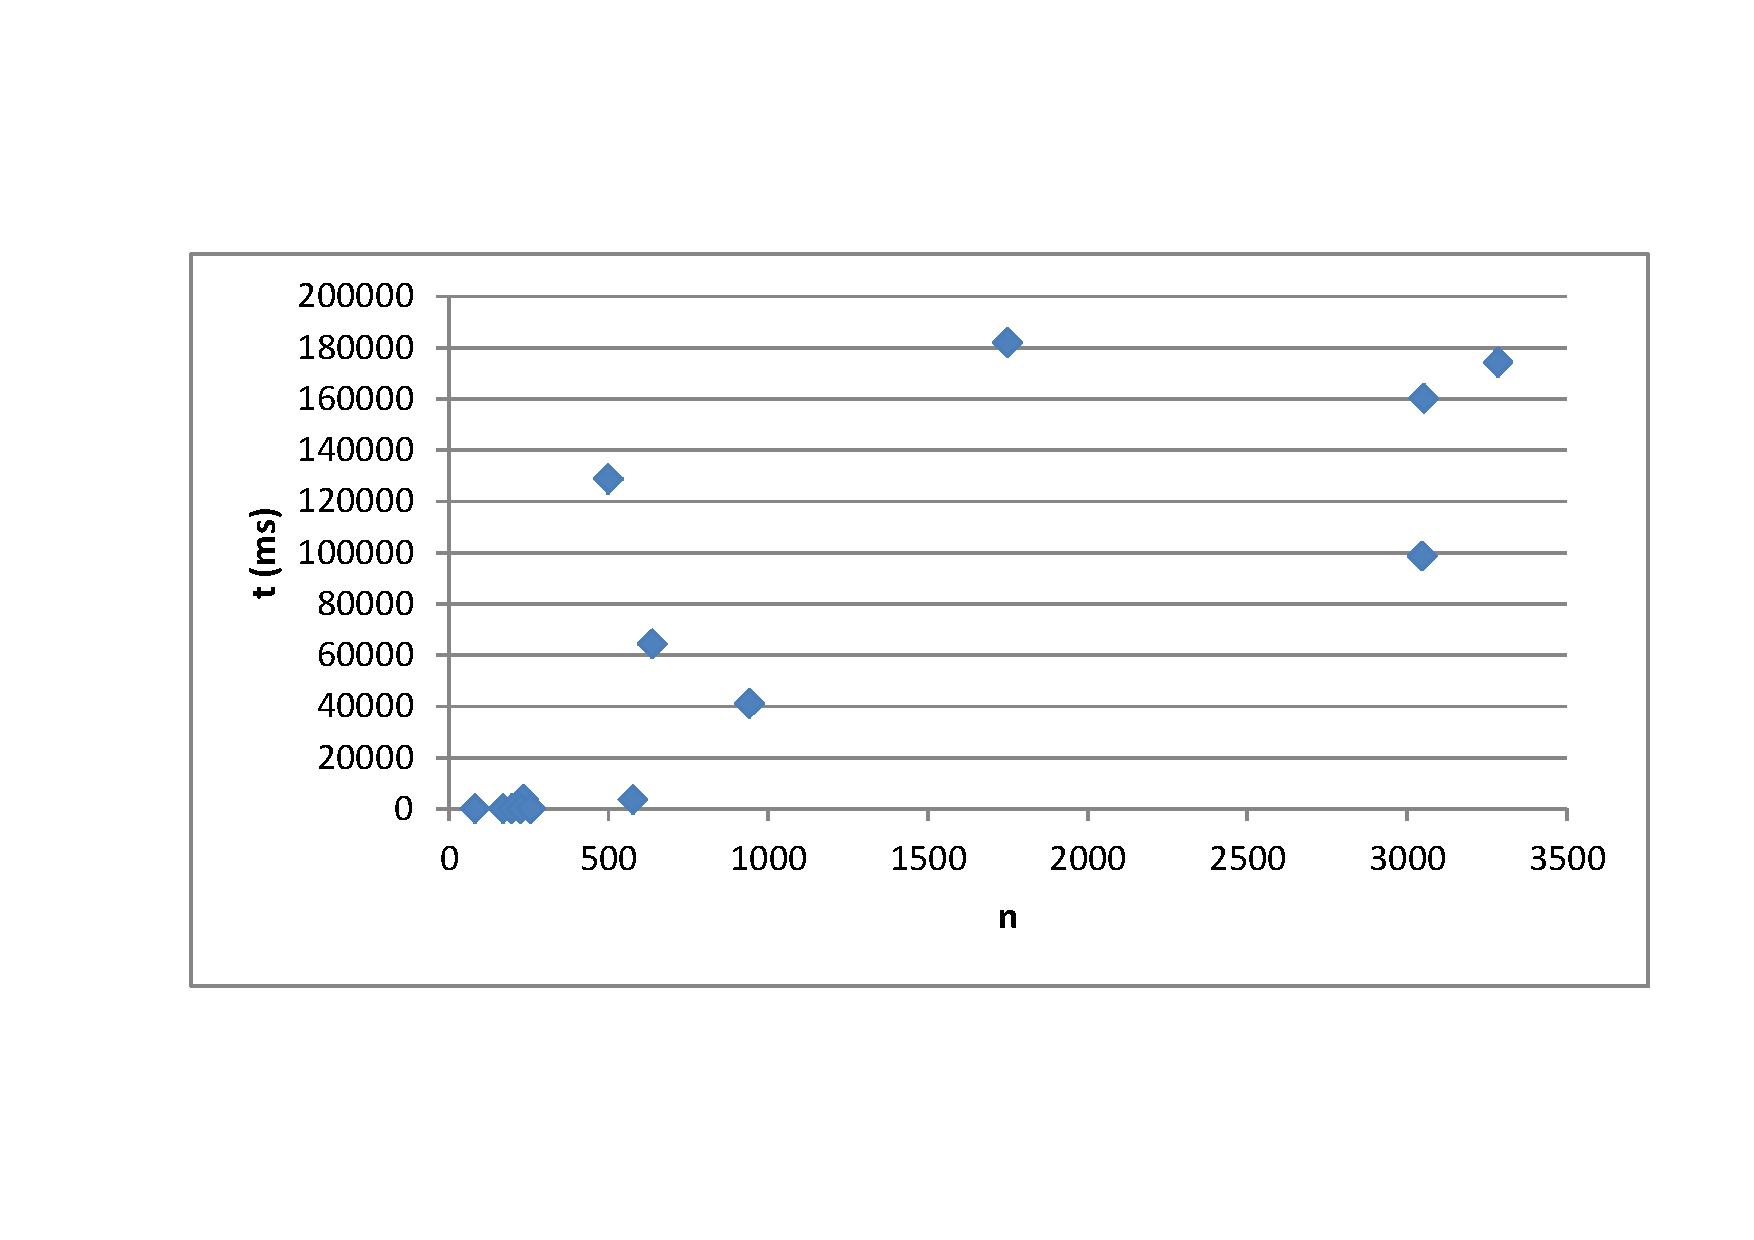
\includegraphics[width=\columnwidth]{../Results/miplib_apache_n.pdf}
\caption{Runtime results for SimplexApache on instances of MIPLIB 2010 \cite{KochEtAl2011} compared to the number of constraints: $n$}
\label{fig:miplibresults_n}
\end{figure}
\begin{figure}[h!]
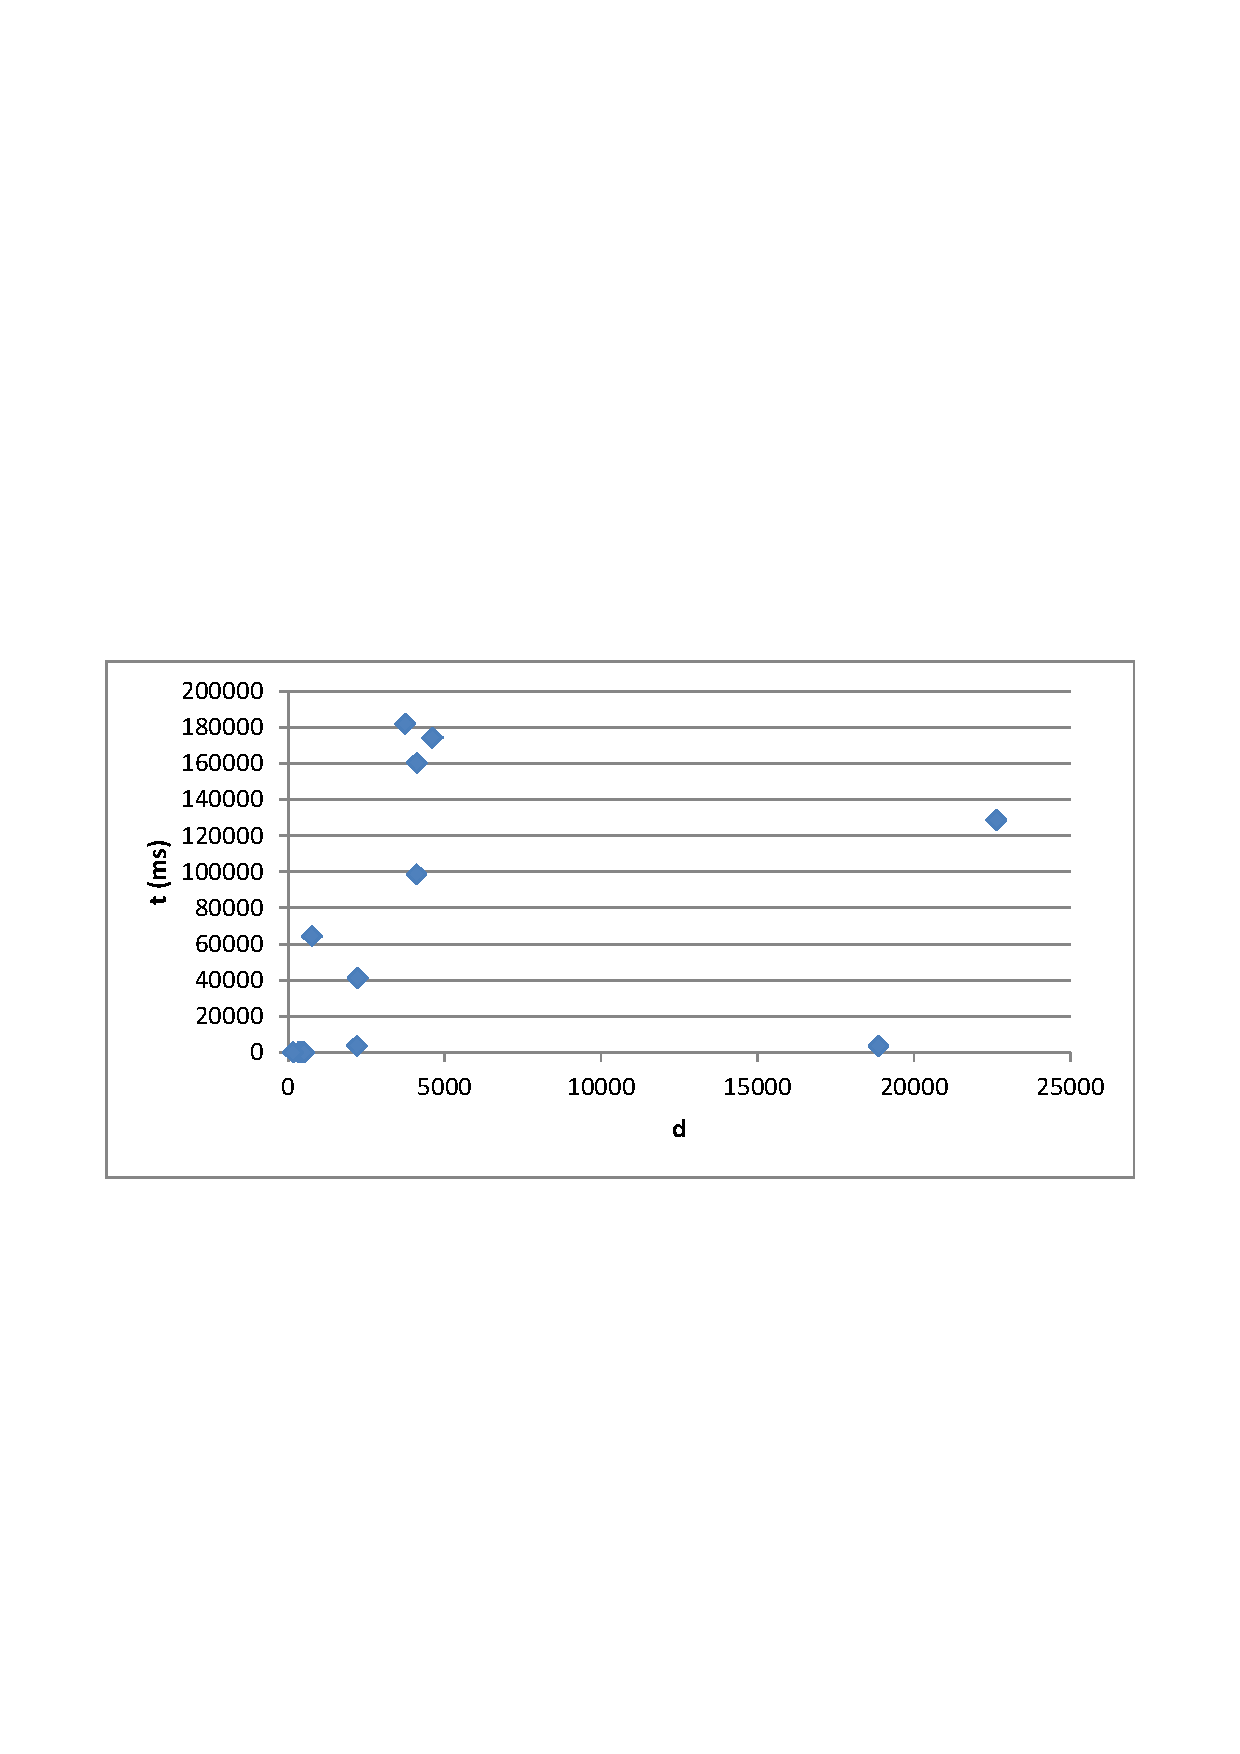
\includegraphics[width=\columnwidth]{../Results/miplib_apache_d.pdf}
\caption{Runtime results for SimplexApache on instances of MIPLIB 2010 \cite{KochEtAl2011} compared to the number of variables: $d$}
\label{fig:miplibresults_d}
\end{figure}

%aantal iteraties binnen simplexApache voor sampleLP & iterSampLP


\section{Analysis of results}
Compare between methods: runtime and asymptotic bounds.

\section{Discussion of the benefit of randomization for the problem}

\section{Conclusions}


\bibliographystyle{abbrv}
\bibliography{sigproc}  % sigproc.bib is the name of the Bibliography in this case
\balancecolumns
\end{document}
